\documentclass[a4paper,12pt]{article}
\usepackage[english,ukrainian,russian]{babel}
\linespread{1}
\usepackage{ucs}
\usepackage[utf8]{inputenc}
\usepackage[T2A]{fontenc}
\usepackage[paper=portrait,pagesize]{typearea}
\usepackage{amsmath}
\usepackage{bigints}
\usepackage{amsfonts}
\usepackage{graphicx}
\usepackage{amssymb}
\usepackage{cancel}
\usepackage{gensymb}
\usepackage{multirow}
\usepackage{booktabs}
\usepackage{rotate} 
\usepackage{pdflscape}
\usepackage{bigstrut}
\usepackage[pageanchor]{hyperref}
\usepackage{chngpage}
\usepackage{fancybox,fancyhdr}
\newcommand\tab[1][1cm]{\hspace*{#1}}
\newcommand{\RomanNumeralCaps}[1]{\MakeUppercase{\romannumeral #1}}
\usepackage[left=20mm, top=20mm, right=15mm, bottom=15mm, nofoot]{geometry}

\usepackage{verbatim}
\usepackage{enumerate}
\usepackage{listings}
\usepackage{xcolor}

\usepackage{mathtools}
\usepackage{MnSymbol}

\definecolor{codegreen}{rgb}{0,0.6,0}
\definecolor{codegray}{rgb}{0.5,0.5,0.5}
\definecolor{codepurple}{rgb}{0.58,0,0.82}
\definecolor{backcolour}{rgb}{0.95,0.95,0.92}

\lstdefinestyle{mystyle}{
	backgroundcolor=\color{backcolour},   
	commentstyle=\color{codegreen},
	keywordstyle=\color{blue},
	numberstyle=\tiny\color{codegray},
	stringstyle=\color{red},
	basicstyle=\ttfamily\footnotesize,
	breakatwhitespace=false,         
	breaklines=true,                 
	captionpos=b,                    
	keepspaces=true,                 
	numbers=none,                    
	numbersep=5pt,                  
	showspaces=false,                
	showstringspaces=false,
	showtabs=false,                  
	tabsize=4,
	frame=shadowbox
}

\lstset{style=mystyle}

% Language "Assembler"
\lstdefinelanguage{assembler}{
    keywords={MOV, LDR, CMP, BEQ, BLT, SUB, B, ADD, STR. DCD, LSL},
    sensitive=true,
    comment=[l]{;},  % Коментарі починаються з ;
    morestring=[b]",  % Рядки в лапках
    morestring=[b]',  % Рядки в одинарних лапках
}
\lstset{
    language=assembler,          % Встановлюємо мову
    basicstyle=\ttfamily,        % Шрифт для коду
    keywordstyle=\color{blue},   % Стиль для ключових слів
    commentstyle=\color{green},  % Стиль для коментарів
    stringstyle=\color{red},     % Стиль для рядків
    numbers=left,                % Номери рядків зліва
    numberstyle=\tiny,           % Стиль номерів рядків
    stepnumber=0,                % Номери для кожного рядка
    numbersep=5pt,               % Відстань до номера рядка
    frame=single,                % Рамка навколо коду
}

\begin{document}
    \pagestyle{fancy}
    \fancyhead{}
    \fancyhead[R]{ФІ-12 Завалій Олександр}
    \begin{center}
        \large{\textbf{Міністерство освіти і науки України\\
                Національний технічний університет України\\
                «Київський політехнічний інститут імені Ігоря Сікорського»\\
                Навчально-науковий Фізико-технічний інститут}}\\
        \hfill \break \hfill \break \hfill\break \hfill \break \hfill \break \hfill \break \hfill \break
        \hfill \break \hfill \break \hfill \break
        \begin{center}
            \normalsize{\textbf{Архітектура комп'ютерних систем\\
            Комп’ютерний практикум\\
            Робота №5}}
        \end{center}
    \end{center}
    \hfill \break \hfill \break \hfill \break \hfill \break \hfill \break \hfill \break \hfill \break
    \hfill \break \hfill \break \hfill \break \hfill \break 
    \begin{flushright}
        \large{ \hspace{35pt} Виконав:\\
            студент групи ФI-12\\
            Завалій Олександр\\} 
        \large{ \hspace{35pt} Перевірив:\\
        Козленко О.В.} 
    \end{flushright}
    \hfill \break \hfill \break \hfill \break \hfill \break \hfill \break \hfill \break \hfill \break
    \hfill \break
    \begin{center} \textbf{Київ-2024} \end{center}
    \thispagestyle{empty}

\newpage
    \begin{center}
        \section*{\bfseries{Робота №5.\\
        Системні виклики в архітектурі x86 на асемблері для операційної системи Linux
    }}
    \end{center}
    \textbf{Мета:} \\
    \hangindent=1.5cm 
    \hangafter=+1 \noindent
    Ознайомитися з роботою системних викликів на мові асемблер в середовищі операційної системи Linux. \\
    \begin{center}  
        \Large{Варіант №4}
    \end{center}
    Зміст індивідуального завдання:
    \begin{table}[h!]
        \centering
        \begin{tabular}{@{}|c|c|c|c|@{}}
        \toprule
        \begin{tabular}[c]{@{}c@{}}Режимом \\ доступу\\ до файлу\end{tabular} & \begin{tabular}[c]{@{}c@{}}Елементи \\ масиву\end{tabular} & \begin{tabular}[c]{@{}c@{}}Операція \\ з масивом\end{tabular}          & \begin{tabular}[c]{@{}c@{}}Системне \\ переривання\end{tabular}     \\ \midrule
        rw-r--rwx                                                             & 8, 5, 3, 6, 7, 12                                          & \begin{tabular}[c]{@{}c@{}}Ділення суми \\ елементів на 2\end{tabular} & \begin{tabular}[c]{@{}c@{}}Створити \\ анонімний  файл\end{tabular} \\ \bottomrule
        \end{tabular}
    \end{table}
    
\newpage
    \begin{center}
        \Large{Code}
    \end{center}
    \begin{lstlisting}[language=assembler]
global _start
section .data
    array db 8,5,3,6,7,12
    arraylen equ 6
    msg db 'My array sum is: ', 0
    msglen equ $-msg
    filename db 'lab5_4', 0
    fract_part db '.5', 0
    fractlen equ $-fract_part

section .bss
    buffer resb 20

section .text
itoa:
    push ebp
    mov ebp, esp
    sub esp, 8
    mov eax, [ebp+8]
    lea edi, [buffer+20]
    mov ecx, 10
    mov dword [ebp-8], 0

.divloop:
    xor edx, edx
    idiv ecx
    add edx, '0'
    dec edi
    mov [edi], dl
    inc dword [ebp-8]
    cmp eax, 0
    jnz .divloop
    mov eax, edi
    mov ecx, [ebp-8]
    leave
    ret

_start:
    mov eax, arraylen
    xor ebx, ebx
    lea ecx, array
    xor edi, edi
    
startloop:
    cmp ebx, eax
    je endloop
    xor edx, edx
    mov dl, [ecx + ebx]
    \end{lstlisting}

\newpage
    \begin{lstlisting}[language=assembler]
    add edi, edx
    inc ebx
    jmp startloop

endloop:
    mov eax, edi
    mov edx, 0
    mov ecx, 2
    div ecx

    push eax
    call itoa
    add esp, 4

    mov eax, 4
    mov ebx, 1
    mov ecx, msg
    mov edx, msglen
    int 0x80

    mov eax, 4
    mov ebx, 1
    mov ecx, buffer
    mov edx, 20
    int 0x80

    cmp edx, 0
    je skip_fraction
    mov eax, 4
    mov ebx, 1
    mov ecx, fract_part
    mov edx, fractlen
    int 0x80

skip_fraction:
    mov eax, 8
    mov ebx, filename
    mov ecx, 0o600
    int 0x80

    mov eax, 15
    mov ebx, filename
    mov ecx, 0o647
    int 0x80  

    mov eax, 356
    mov ebx, filename
    mov ecx, 1
    int 0x80
    \end{lstlisting}

    \newpage
    \begin{lstlisting}[language=assembler]
    mov eax, 1
    xor ebx, ebx
    int 0x80
    \end{lstlisting}

    \begin{center}
        \Large{Results}
    \end{center}
    \begin{figure}[h!]
        \begin{minipage}[h]{1\linewidth}
            \centering
            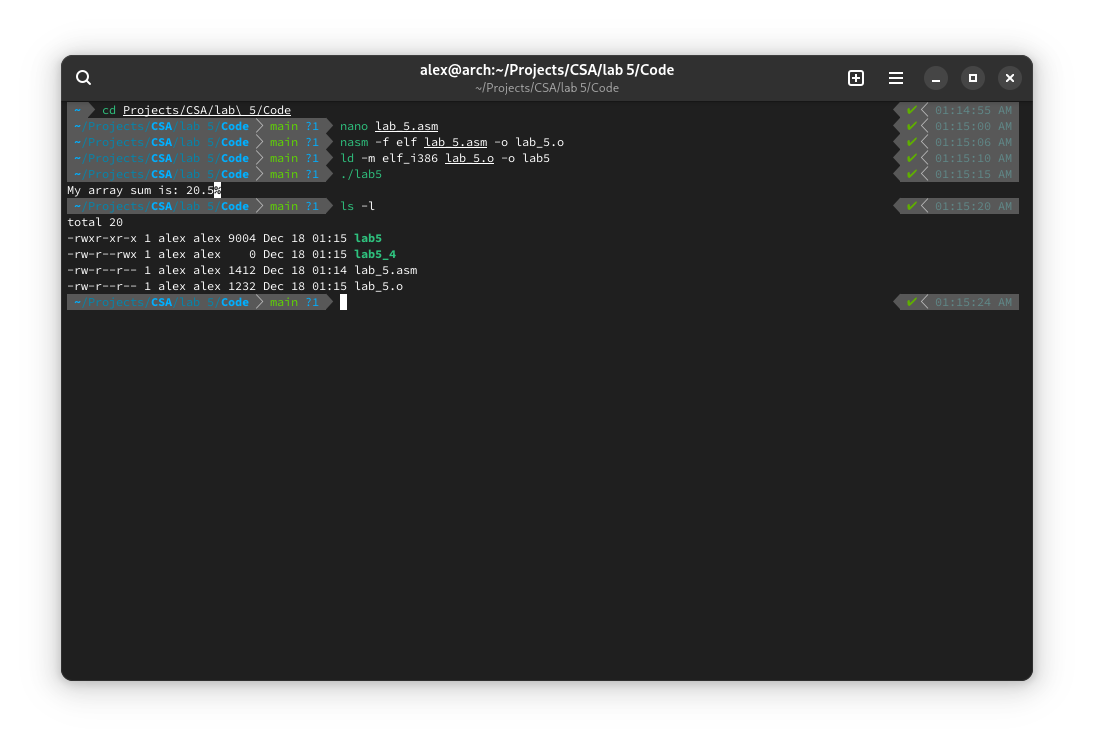
\includegraphics[width=1\linewidth]{Prt sc/figure_1.png}  
        \end{minipage}
    \end{figure}
    За допомогою утиліти strace можемо відслідкувати взаємодію нашої програми та ядра лінукс.
    В результаті бачимо рядок \textbf{memfd\_create("lab5\_4", MFD\_CLOEXEC) = 4}. Розберемо параметри:
    \begin{itemize}
        \item \textbf{memfd\_create} — створює анонімний файл у пам'яті із назвою lab5\_4 та прапором MFD\_CLOEXEC.
        Цей файл буде автоматично закрито при виконанні \textbf{execve}.
        \item \textbf{= 4} — файловий дескриптор файлу.
    \end{itemize}
    Анонімний файл, який ми створили за допомогою \textbf{memfd\_create} не має імені у файловій системі.
    Проте має файловий дескриптор, який повертається системним викликом у регістрі \textbf{eax}. 
    Цей дескриптор можемо використовувати для операцій з файлом.

\end{document}